\section{kMaX-DeepLab模型}

% \subsection{背景}
\par kMaX-DeepLab\cite{kmeans_mask_transformer}是由Google联合约翰霍普金斯大学,在ECCV 2022的论文中提出的一种新的图像全景分割模型。
它分析了现有Transformer模型结构在图像识别任务上的弊端,提出使用kMaX解码器来替换Transformer中的解码器,不仅可以生成更合理的注意力图,而且还具有更好的性能。

\subsection{模型特征}

\par 如图\ref{fig:kmaxdeeplab}\cite{kmeans_mask_transformer}所示,kMaX-DeepLab 主要由三个组件构成,包含像素编码器(Pixel Encoder)、增强像素解码器(Enhanced Pixel Decoder)和 kMaX 解码器。

\begin{enumerate}
	\item 像素编码器使用任意的卷积神经网络(CNN)或Transformer主干,负责从输入图像中提取视觉特征,输出一个特征映射(Feature Maps),代表输入图像的高级语义信息。
	\item 增强像素解码器通过使用一系列的上采样层和卷积层,将像素编码器的特征映射上采样并恢复到输入图像的高分辨率。它输出一个特征映射,代表输入图像的像素级细节。
	\begin{figure}[htbp]
		\centering
		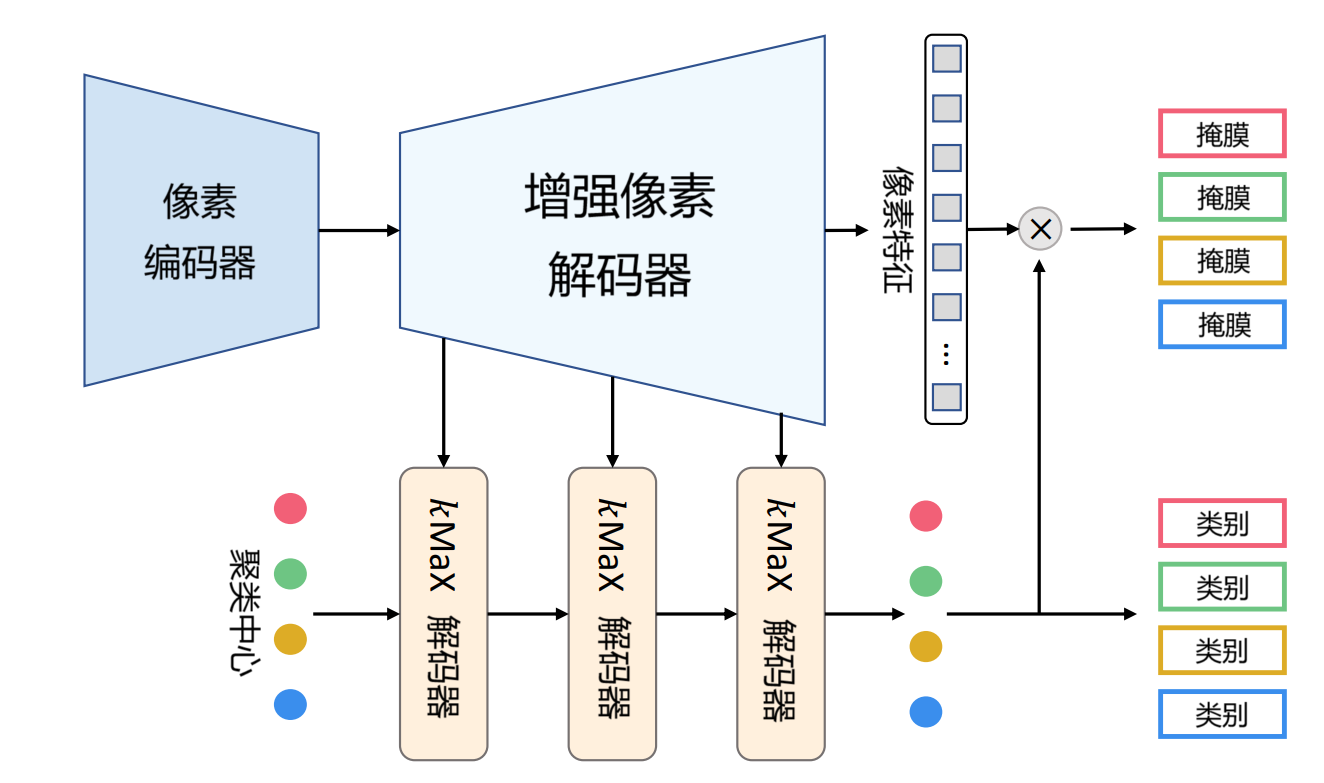
\includegraphics[width=0.9\textwidth]{figures/kmax_deeplab.png}
		\caption{kMaX-DeepLab 架构}
		\label{fig:kmaxdeeplab}
	\end{figure}
	\item kMaX 解码器负责将目标查询向量(如聚类中心)通过K-Means聚类转换成掩膜嵌入向量(Mask Embedding Vectors),如图\ref{fig:kmaxdecoder}\cite{kmeans_mask_transformer}所示。它会为每个目标查询向量输出一个掩膜嵌入向量,用来生成最终的分割掩膜。
	\begin{figure}[htbp]
		\centering
		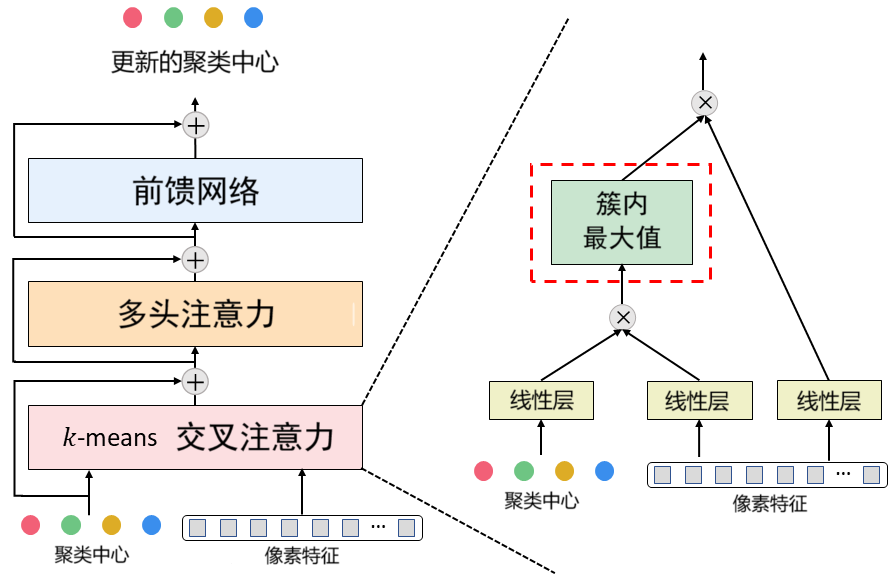
\includegraphics[width=0.9\textwidth]{figures/kmax_decoder.png}
		\caption{kMaX 解码器}
		\label{fig:kmaxdecoder}
	\end{figure}
\end{enumerate}

\subsection{注意力(Attention)机制}

\par 原始的 Mask Transformer(MaX-DeepLab)\cite{mask_transformer} 中的交叉注意力(Cross-Attention)机制使用空间(Spatial-Wise)Softmax 计算查询(Queries)和像素之间的相似度。这种方法有两个主要缺点:

\begin{enumerate}
	\item 计算量大,因为它需要对查询特征图(Object Queries)中的每个空间位置进行 Softmax 操作。
	\item 结果不准确,因为 Softmax 操作会平滑注意力的权重,使得区分重要性的特征变得模糊。
\end{enumerate}

\par kMaX-DeepLab 在 MaX-DeepLab\cite{mask_transformer} 和 CMT-DeepLab(Clustering Mask Transformer)\cite{cluster_mask_transformer} 像素簇聚类过程(图\ref{fig:cluster_mask_transformer})的基础上,提出了通过使用 K-Means 交叉注意力来解决这些问题,将 Mask Transformer\cite{mask_transformer}视为迭代执行聚类分配和聚类更新的过程。K-Means 交叉注意力首先将查询特征图聚类为固定数量的簇(Cluster)。然后通过找到最接近簇质心的关键特征图来计算每个簇的注意力权重。
这种方法比空间 Softmax 更高效,因为它只需要对整个查询特征图进行一次 K-Means 聚类操作。其次,这种方法也更准确,因为注意力权重不会被 Softmax 操作平滑。
因此,kMaX-DeepLab 的速度是原始 Mask Transformer 的3倍,在 Cityscapes 数据集上的准确率比原始 Mask Transformer 高出1.5\%。此外,kMaX-DeepLab 对噪声和离群值更具鲁棒性,训练效率更高,并且可以与其他注意力机制(如自注意力 Self-Attention)一起使用。

\begin{figure}[htb]
	\centering
	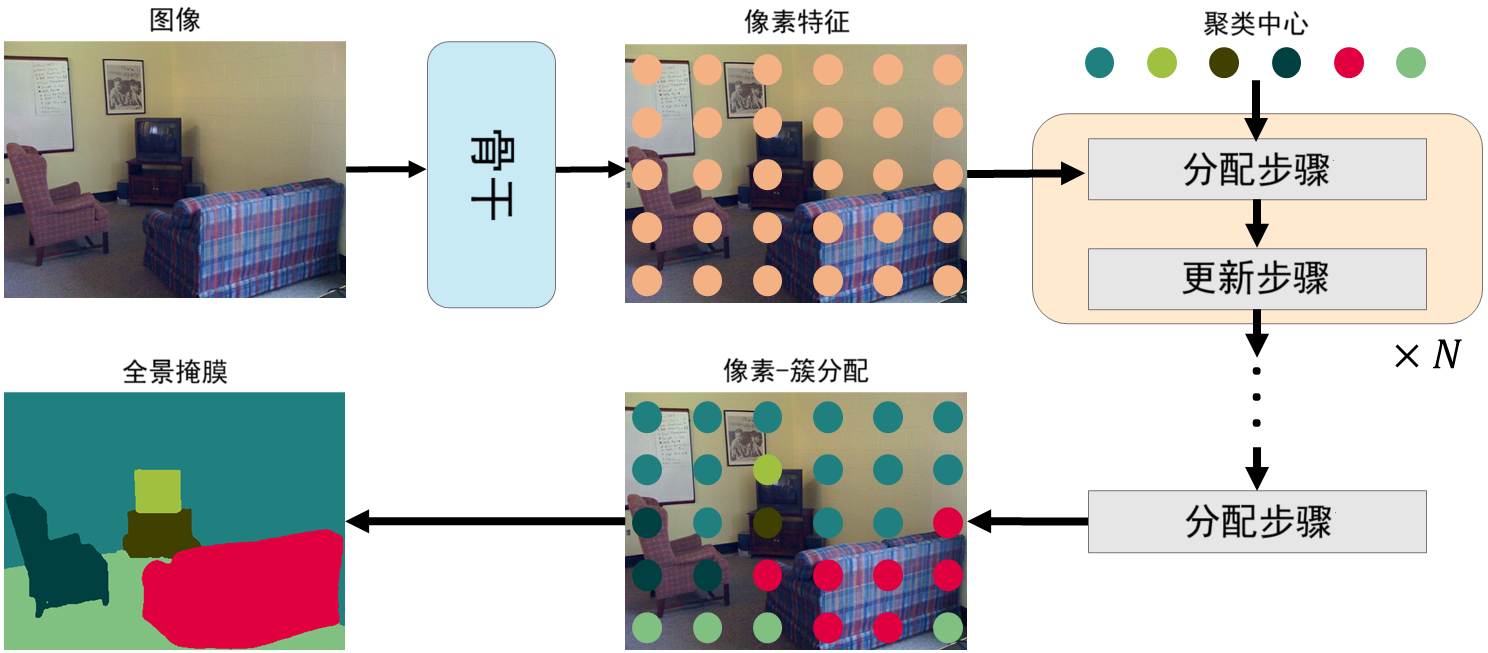
\includegraphics[width=0.9\textwidth]{figures/clustering_view_of_mask_transformer.png}
	\caption{CMT-DeepLab 像素簇聚类过程}
	\label{fig:cluster_mask_transformer}
	\note{注:CMT层根据特征相似度将像素分配给各个聚类中心,用于更新像素特征和聚类中心。经过多个 CMT 层后,获得精细的像素簇分配,产生最终的全景掩模。}
\end{figure}

% \subsection{模型效果}

% \par 如表\ref{seg model accuracy}所示,kMaX-DeepLab 在多种基准测试中都取得了最佳结果\cite{kmeans_mask_transformer}。在 COCO 数据集上的全景分割质量(panoptic quality,PQ)得分为58.0\%;在 Cityscapes 数据集上的 PQ 得分为68.4\%,精确率(average precision,AP) 得分为44.0\%,平均交并比(mean Intersection over Union,mIoU)
% 得分为83.5\%;在 ADE20K 数据集上的 PQ 得分为50.9\%,mIoU 得分为55.2\%。相对于先前的模型均产生了巨大的进步,
% 展示了基于 Transformer 的架构在全景分割方向的潜力。

% \begin{table}[htb]
% 	\centering
% 	\caption{全景分割模型测试结果}
% 	\label{seg model accuracy}
% 	\begin{tabular}{ccccc}
% 		\toprule
% 		Model              & backbone            & COCO $\text{PQ}^{\text{all}}$ & COCO $\text{PQ}^{\text{things}}$ & COCO $\text{PQ}^{\text{stuff}}$ \\
% 		\midrule
% 		kMaX-DeepLab       & ConvNeXt-L          & 58.1                          & 64.3                             & 48.8                            \\
% 		MaskFormer         & Swin-L (W12)        & 57.8                          & 64.2                             & 48.1                            \\
% 		Panoptic SegFormer & Swin-L (W7)         & 55.8                          & 61.7                             & 46.9                            \\
% 		CMT-DeepLab        & Axial-R104-RFN      & 55.3                          & 61.0                             & 46.6                            \\
% 		\toprule
% 		Model              & backbone            & Cityscapes PQ                 & ADE20K AP                        & ADE20K mIoU                     \\
% 		\midrule
% 		kMaX-DeepLab       & ConvNeXt-L          & 68.4                          & 44.0                             & 83.5                            \\
% 		Mask2Former        & Swin-L (W12)        & 66.6                          & 43.6                             & 82.9                            \\
% 		Axial-DeepLab      & Axial-ResNet-XL     & 64.4                          & 36.3                             & 80.6                            \\
% 		Panoptic-DeepLab   & SWideRNet-(1,1,4.5) & 66.4                          & 40.1                             & 82.2                            \\
% 		\bottomrule
% 	\end{tabular}
% \end{table}